

%!TEX root = ../Notes.tex
\chapter{Distinguishing Spaces} 
\begin{definition}
	A \textbf{topological property} (or `top. prop.') is a property of a topological spaces that is preserved by homeomorphisms. 
\end{definition}
\begin{center}
	\textbf{List of Topological Properties thus Far} 
\end{center}
\begin{enumerate}
	\item Cardinality of $X$ 
	\item Cardinality of $F_x$ 
	\item Metrizability (we proved this in the homework) 
	\item Discreteness 
	\item Indiscreteness 
\end{enumerate}
\begin{lemma}
	[Rachel's Lemma] Let $(X, F_X) $ and $(Y, F_Y)$ be topological spaces and $f: X \rightarrow Y$ be an open bijection. If $F_X$ is the discrete topology, then $F_Y$ is the discrete topology. 
\end{lemma}
\begin{proof}
	Let $y \in Y$. Since $f$ is surjective, there exists $x \in X$ such that $f(x) = y$. Since $\{x\} \in F_X$ and $f$ open, $f(\{x\}) \in F_Y$. Thus all singletons in are elements of $F_Y$ and all sets in $Y$ are unions of singletons and hence elements of $F_Y$, so every set is an open set and $F_Y$ is the discrete topology. 
\end{proof}
\begin{lemma}
	[Daniel's Lemma] Let $(X, F_X) $ and $(Y, F_Y)$ be topological spaces and $f: X \rightarrow Y$ be a continuous bijection. If $F_X$ is the indiscrete topology, then $F_Y$ is the indiscrete topology. 
\end{lemma}
\begin{proof}
	Let $U \in F_Y$. WTS $U = Y$ or $U = \emptyset$. Since $f$ is continuous, $f^{-1}(U) \in F_X$. Therefore $f^{-1}(U) = X$ or $\emptyset$. \\
	Suppose $f^{-1}(U) = X$. Then $U = f(f^{-1}(U)) = f(X) = Y$ since $f$ surjective.\\
	Suppose $f^{-1}(U) = \emptyset$. Then $U = \emptyset$. Therefore $F_Y$ is the indiscrete topology. 
\end{proof}

Corollaries: If $(X, F_X) $ and $(Y, F_Y)$ topological spaces and $f: X \rightarrow Y$ a homeomorphism, then 
\begin{enumerate}
	\item $F_X$ the discrete topology $\Longrightarrow$ $F_Y$ the discrete topology 
	\item $F_X$ the indiscrete topology $\Longrightarrow$ $F_Y$ the indiscrete topology 
\end{enumerate}

Unfortunately, even with these five lovely Topological Properties, we can't yet distinguish a circle from a line. Clearly there is more work to do. 
\begin{example}
	[a non-example] Distance is not a topological property. A big circle \emph{is} homeomorphic to a little circle. 
\end{example}

\section{Compactness} 
\begin{definition}
	Let $(X, F_X)$ be a topological space and $S \subseteq X$.\\
	We say $\{U_j : j \in J\}$ is an $\mathbf{open \ cover}$ of $S$ if for all $j \in J$, $U_j \in F_X$ and $S \subseteq \bigcup_{j \in J}U_j$.\\
	We say $\{U_j : j \in K\}$ is a \textbf{subcover} if $K \subseteq J$ and $S \subseteq \bigcup_{j \in K} U_j$.
	
	We say $S$ is \textbf{compact} if every open cover of $S$ has a finite subcover. 
\end{definition}

\textbf{IMPORTANT WARNING!}\\
We learned in Math 131 that in $\R^{n}$, a set if compact $\Longleftrightarrow$ it is closed and bounded. THIS IS NOT TRUE IN TOPOLOGICAL SPACES. DO NOT TRY TO USE IT. 
\begin{example}
	Is the set $(0,1)$ compact in 
	\begin{enumerate}
		\item $\R$ with the discrete topology? 
		\item $\R$ with the half-open topology? 
		\item $\R$ with the finite complement topology? 
	\end{enumerate}
\end{example}

Answers: 
\begin{enumerate}
	\item No. Take the open covering $\{B_{1/2}(x) : x \in (0,1)\}$. If we remove any of these balls, the corresponding $x$ will no longer be covered. However, there are clearly uncountably infinitely many balls. \\\\
	\item No. Take the open covering $\{[\frac{1}{n}, 1) : n \in \N\}$ so that $(0,1) = \bigcup_{n \in \N}([\frac{1}{n}, 1)$. There is not finite subcover. \\\\
	\item Yes. Suppose we have a cover of $(0,1)$. Take any element of the cover, say $U_{47}$. $U_{47}$ is missing at most finitely may elements of $(0,1)$ since its complement is finite. For each element $x \in \R \setminus U_{47}$, select one $U_{j_x}$ containing $x$. The set $\{U_{47}\} \cup \{U_{j_x}: x \in \R \setminus U_{47}\}$ is a finite open subcover. 
\end{enumerate}
\begin{theorem}
	[analogous to a theorem from 131] Let $(X, F_X)$ and $(Y, F_Y)$ be topological spaces, $S \subseteq X$, and $f : X \rightarrow Y$ continuous. If $S$ is compact then $f(S)$ is compact. 
\end{theorem}
\begin{proof}
	\begin{enumerate}
		\item Take a covering of $f(S)$. 
		\item Applying $f^{-1}$ to these sets, we pull back to an open covering of $S$. 
		\item Take a finite subcover. 
		\item Push these forward again. We have a finite cover of $f(S)$. 
	\end{enumerate}
\end{proof}

As a corollary we have \textbf{Topological Property 6: Compactness}.\\
\begin{theorem}
	Any closed subset of a compact space is compact. 
\end{theorem}
\begin{proof}
	\begin{enumerate}
		\item Take an open cover of $S$ 
		\item Add $X \setminus S$. Now we have an open cover of $X$. 
		\item Take a finite subcover. 
		\item Remove $X \setminus S$. Not we have a finite subcover of $S$. 
	\end{enumerate}
\end{proof}
\begin{theorem}
	[also analagous to a 131 theorem] Let $(X, F_X)$ be compact and $f : X \rightarrow \R$ be continuous. Then $f$ has a max value and a min value. 
\end{theorem}
\begin{proof}
	\begin{enumerate}
		\item $f(X)$ is compact by Analogous Theorem 1 
		\item Therefore $f(X)$ is closed and bounded 
		\item Therefore $f(X)$ has a lub and a glb (ie a max and a min) 
	\end{enumerate}
\end{proof}
\begin{smallfact}
	Let $(X, F_X)$ be a topological space. Suppose every open cover of $S \subseteq X$ made up of basis elements has a finite subcover. Then $X$ is compact. 
\end{smallfact}
\begin{proof}
	Let $\{U_j : j \in J\}$ be an open cover of $S$ and $\beta$ be a basis of $S$. For every $j \in J$, $U_j = \bigcup_{i \in I_j}B_i$ where for every $i \in I_j$ $B_i \in \beta$. Hence $\{B_i : i \in I_j \text{ and } j \in J\}$ is an open cover of $S$. By hypothesis, we have a finite subcover, $\{B_i : i \in K_j \text{ and } j \in K\}$ where $K \subseteq J$ and $K$ is finite, and for all $j \in K$, $K_j \subseteq I_j$ and $K_j$ is finite. Now note that given any $j \in K$, for every $i \in K_j$ $B_i \subseteq U_j$. Hence
	\[X = \bigcup_{j\in K} \left[ \bigcup_{i \in K_j} B_i \right] \subseteq \bigcup_{j\in K} U_j \subseteq X\]
	and $\{U_j : j\in K\}$ is a finite subcover. 
\end{proof}
\begin{theorem}
	[Bolzano-Weierstrass Theorem] Let $(X,F_X)$ be a compact topological space. Then for all infinite $S \subseteq X$, $\exists \ p \in X$ such that $\forall \ U \in F_X$ with $p \in U$, $U$ contains infinitely many points of $S$. 
\end{theorem}
\begin{proof}
	Suppose that for some such $S \subseteq X$, no such $p \in X$ exists. Therefore, for all $p \in X$ there exists some $U_p \in F_X$ such that $p \in U_p$ and $|S \cap U_p|$ is finite. So, as $\displaystyle{\bigcup_{p \in X} U_p = X}$, $\{U_p \mid p \in X\}$ is an open cover of $X$. As $X$ is compact, there exists some finite subcover $\{U_{p_1},...,U_{p_n}\}$. Hence, from the definition of a subcover, $\displaystyle{X = \bigcup_{i=1}^n U_{p_i}}$. Intersecting both sides with $S$ gives that:
	\[S = \left(\bigcup_{i=1}^n U_{p_i}\right) \cap S = \bigcup_{i=1}^n (U_{p_i} \cap S)\]
	However, as $|U_p \cap S|$ is finite for all $p \in X$, $|U_{p_i} \cap S|$ is finite for $1 \leq i \leq n$. The union of finite sets is finite, and therefore $\left|\bigcup_{i=1}^n (U_{p_i} \cap S)\right|$ is finite. However, $S$ is infinite by assumption. So this is a contradiction, and no such $S$ exists. 
\end{proof}
\begin{theorem}
	[Finite Tychonoff Theorem] Let $(X,F_X)$ and $(Y,F_Y)$ be compact topological spaces. Then $(X \times Y, F_{X \times Y})$ is also a compact topological space. 
\end{theorem}
\begin{proof}
	{(Comic book style)}
	\begin{figure}
		[h!] 
		\begin{center}
			\subfigure[Consider some open cover.]{
			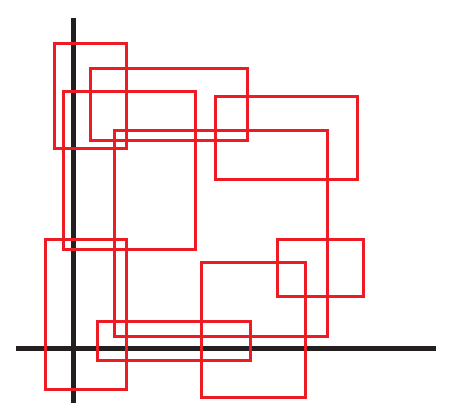
\includegraphics[width=190pt]{images/compactness/tychonoff_comic_1}} \subfigure[Restrict to some $\{x\} \times Y$, which is compact, so has a finite subcover.]{
			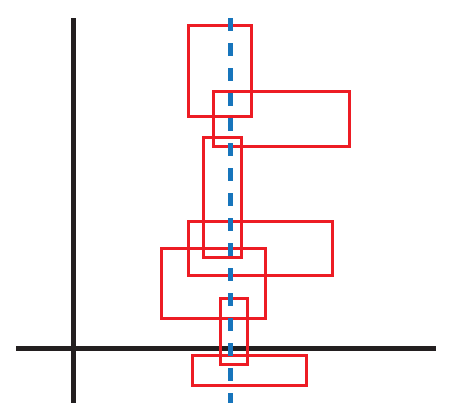
\includegraphics[width=190pt]{images/compactness/tychonoff_comic_2}} 
		\end{center}
	\end{figure}
	\pagebreak 
	\begin{figure}
		[h!] 
		\begin{center}
			\subfigure[So there is some open $U_x$ with $x \in U_x$ s.t. $U_x \times Y$ is contained in this subcover.]{
			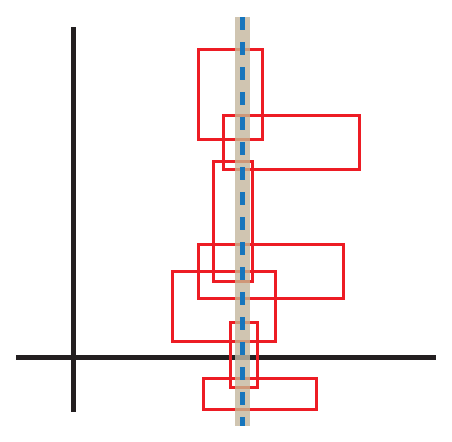
\includegraphics[width=190pt]{images/compactness/tychonoff_comic_3}} \subfigure[So consider just the $U_x$, which are a cover of $X$, so have a finite subcover.]{
			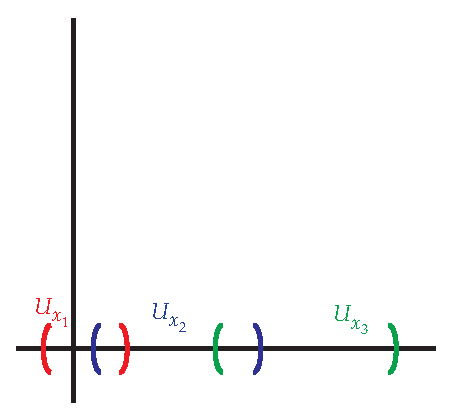
\includegraphics[width=190pt]{images/compactness/tychonoff_comic_4}} 
		\end{center}
	\end{figure}
	
	So the original sets that covered $\{x\} \times Y$ corresponding to the chosen $U_x$ for the desired finite cover of $X \times Y$. 
\end{proof}
Now let's do a real proof. 
\begin{proof}
	{(Real)} Consider an open cover of $X \times Y$ consisting of basis elements, $\{U_i \times V_i \mid i \in I\}$, where $U_i \in F_X$ and $V_i \in F_Y$ for all $i \in I$.
	
	Let $x \in X$. It is clear that $\{x\} \times Y \cong Y$, so $\{x\} \times Y$ is compact. So the original open cover is a cover of $\{x\} \times Y$, and there exists some finite subcover $\{U_{i(x)} \times V_{i(x)} \mid i(x) \in K_x\}$ where $K_x \subseteq I$ and $K_x$ is finite. If $x \notin U_{i(x)}$, removing the set $U_{i(x)} \times V_{i(x)}$ does not change the fact that the remaining set is a finite subcover of $\{x\} \times Y$. Hence, without loss of generality, we assume that $x \in U_{i(x)}$ for all $i(x) \in K_x$.
	
	Next, define $\displaystyle{U_x = \bigcap_{i(x) \in K_x} U_{i(x)}}$. As $U_{i(x)} \in F_X$ for all $i(x) \in K_x$, $U_x$ is the intersection of finitely many open sets, and so is open. Additionally, as $x \in U_{i(x)}$ for all $i(x) \in K_x$, $x \in U_x$.
	
	Claim 1: $\{U_x \times V_{i(x)} \mid i(x) \in K_x\}$ is an open cover of $\{x\} \times Y$.
	
	Proof: Let $(x,y) \in \{x\} \times Y$. Then for some $i(x) \in K_x$, $(x,y) \in U_{i(x)} \times V_{i(x)}$. So $y \in V_{i(x)}$. Then, as $x \in U_x$, $(x,y) \in U_x \times V_{i(x)}$. As such an $i(x) \in K_x$ exists for all $(x,y) \in \{x\} \times Y$, $\{U_x \times V_{i(x)} \mid i(x) \in K_x\}$ is an open cover of $\{x\} \times Y$.
	
	Now, as $x \in U_x$ and $U_x \in F_X$ for all $x \in X$, $\{U_x \mid x \in X\}$ is an open cover of $X$. As $X$ is compact, this must have a finite subcover, $\{U_x \mid x \in L\}$, where $L \subseteq X$ and $L$ is finite.
	
	Claim 2: $\{U_x \times V_{i(x)} \mid x \in L, i(x) \in K_x\}$ is a cover of $X \times Y$.
	
	Proof: Let $(x_0,y_0) \in X \times Y$. As $\{U_x \mid x \in L\}$ covers $X$, there exists some $x \in L$ such that $x_0 \in U_x$. As $\{U_x \times V_{i(x)} \mid i(x) \in K_x\}$ covers $\{x\} \times Y$, there exists some $i(x) \in K_x$ such that $(x,y_0) \in U_x \times V_{i(x)}$, so $y_0 \in V_{i(x)}$. Hence $(x_0, y_0) \in U_x \times V_{i(x)}$, and $(x_0,y_0)$ is in the cover. As this holds for all such $(x_0,y_0) \in X \times Y$, $\{U_x \times V_{i(x)} \mid x \in L, i(x) \in K_x\}$ is a cover of $X \times Y$.
	
	Claim 3: $\{U_{i(x)} \times V_{i(x)} \mid x \in L, i(x) \in K_x\}$ is a cover of $X \times Y$.
	
	Proof: Let $(x_0,y_0) \in X \times Y$. As $\{U_x \times V_{i(x)} \mid x \in L, i(x) \in K_x\}$ is a cover of $X \times Y$, there exists some $x \in L$, $i(x) \in K_x$ such that $(x_0,y_0) \in U_x \times V_{i(x)}$. From the definition of $U_x$, $U_x \subseteq U_{i(x)}$. Therefore, as $x_0 \in U_x$, $x_0 \in U_{i(x)}$, and $(x_0, y_0) \in U_{i(x)} \times V_{i(x)}$. As such a $x \in L$, $i(x) \in K_x$ exists for all $(x_0, y_0) \in X \times Y$, this is a cover of $X \times Y$. 
	
	Finally, let $J = \bigcup_{x \in L} K_x$. As $L$ is finite, and $K_x$ is finite for all $x \in X$, $J$ is finite. Additionally, as $K_x \subseteq I$ for all $x \in X$, $J \subseteq I$. So $\{U_i \times V_i \mid i \in J\}$ is a finite subcover of $\{U_i \times V_i \mid i \in I\}$. Also, as this has $\{U_i \times V_i \mid i \in J\} = \{U_{i(x)} \times V_{i(x)} \mid x \in L, i(x) \in K_x\}$, this is a cover of $X \times Y$.
	
	So $\{U_i \times V_i \mid i \in J\}$ is a finite subcover of $X \times Y$. As such a subcover exists for any cover of basis elements, $X \times Y$ is compact. 
\end{proof}
